\documentclass[times, 10pt,onecolumn]{article} 
\usepackage{latex8}
\usepackage{times}
\usepackage{url}
\usepackage{graphicx}
\usepackage{amsmath}
%\usepackage{amsfonts, amsthm}

\title{Artificial Intelligence in Software Engineering}
\author{
Xusheng Xiao\\
\small{xxiao2@ncsu.edu}\\
}
\date{April 23, 2011}


\newcommand{\N}{\mathbb{N}}
\newcommand{\Z}{\mathbb{Z}}
\newcommand{\R}{\mathbb{R}}

\begin{document} 
\maketitle
\thispagestyle{empty}
\pagestyle{empty}

\begin{abstract}
Software Engineering is a knowledge-intensive activity, presumably requiring intelligence. To reduce human efforts in the activities of software engineering, Artificial Intelligence (AI) techniques, which aims to create computer systems that exhibit some form of human intelligence, are employed to assist or automate various activities of software engineering, such as testing, program analysis, debugging and even self-repair. In this project, I will provide a study of how various AI techniques are used in automating or assisting various activities of software engineering. In this report, we provide the details on how AI can be used in assisting software testing, fault detection and software repair. 
\end{abstract}
\section{Introduction} 
Software Engineering is a knowledge-intensive activity, presumably requiring intelligence. Many software engineering activities, such as testing, analysis and debugging, require intensive human intelligence and are error-prone. To reduce human efforts in the activities of software engineering, Artificial Intelligence (AI) techniques, which aims to create computer systems that exhibit some form of human intelligence, are employed to assist or automate various activities of software engineering, such as testing, program analysis, debugging and even self-repair. In this report, we present the details of the application of AI in software engineering and provide a detailed survey of the existing tools and techniques associating with AI in three important software engineering activities: testing,
fault detection and software repair.

Over the past decades, many AI techniques are applied to assist automated software testing, such as constraint solving~\cite{constraintsolving} used in Dynamic Symbolic Execution~\cite{symbolic, dart, cute} for test-input generation, heuristics used to prune search space of test-generation tools~\cite{prune,fitness}, and machine learning used in statistical software testing~\cite{mlinstatistics} and coverage prediction of testing tools~\cite{predictCoverage}. In this report, we provide the details on test generation using symbolic execution and pruning search space of symbolic execution using heuristics.

As the size of complexity of software has grown quickly in past decades, the difficulty of finding and fixng bugs has increased. Recent research works~\cite{wrongDefinition,online} that use AI techniques have advanced the research in reducing the human efforts on fault detection: Shi et al.~\cite{wrongDefinition} proposes an approach to first learn the Definition-Use Invariants and then use the learned knowledge of Definition-Use for detecting concurrency and sequential bugs; Baah et al~\cite{online} and proposes a new machine-learning technique that performs fault detection for deployed software. I plan to study in details how these research works adopt the concepts and techniques of AI to assist the task of fault detection.

By adapting the well-known AI techniques, even the most challenging tasks, debugging and self-repair, can be half or even full automated. Genetic programming, an evolutionary algorithm-based methodology in AI, is used and adapted by Weimer et al.~\cite{geneticPatch}' approach to automatically find patches for programs and automatically fix bugs~\cite{repair}. Inspired by these works, Schulte et al. further propose an approach to study the evolution of assembly code~\cite{evolutionaryComputation} for automated program repair. I plan to investigate these techniques to study how AI can achieve automated software repair.






\section{AI in Software Testing}
To achieve automatic test (data) generation from source code, there exists a well established framework: constraint-based testing~\cite{constraint,inka,dart,cute,onthefly}  (CBT). CBT approach focuses on translating part of a program into a logical formula whose solutions are relevant to test data. CBT also can be global, translating the whole program in a formula \cite{constraint,inka}, or local (path-based) \cite{dart,cute,onthefly}, focusing on a single path. In this report, we focus on path-based CBT, referred as path-based testing. 

Symbolic execution~\cite{symbolic} is a way to track programs symbolicly rather than executing them with actual input value. Concolic path-based testing tools have literally blossomed up recently \cite{extenjpf,structural,mixed,exe,fuzz,pex} with the impressive progress in constraint solvers. Concolic path-based testing tools combine both concrete and symbolic execution (referred as concolic execution~\cite{dart,cute} or mixed execution~\cite{mixed}), which makes it possible to perform automatic path-based testing on large scale programs. By executing the program under test with concrete values while performing symbolic execution, symbolic constraints on the inputs can be collected from the predicates in branch statements, forming an expression, called path condition. To explore new paths, part of the constraints in the collected path conditions are negated to obtain new path conditions, which are sent to a constraint solver to compute test inputs for new paths. In theory, all feasible execution paths will be exercised eventually through the iterations of constraint collection and constraint solving in DSE. 

A program under test can be modelled as a control flow graph (CFG)~\cite{testbook}, whose nodes represent simple primitive statements (such as input, output, and assignment) and edges represent the flow of control. An execution path of the program is a path on CFG from the starting node, entry of the program, to the exit node, exit of the program. Thus, to explore all paths of the program under test, i.e. achieving 100\% path coverage, is to enumerate all paths between two nodes in a graph, which is well known as a NP-hard problem~\cite{graph}. To alleviate this path explosion problem and to reduce the computation complexity, different AI techniques has been proposed, such as pruning search space of symbolic execution using heuristics~\cite{prune}, selective symbolic execution~\cite{selective} and fitness-guided path exploration~\cite{fitness}. In this report, we provide the details on pruning search space of symbolic execution using heuristics.

Recent and impressive progress in constraint solvers as well as the combination of both concrete and symbolic execution (referred as concolic execution~\cite{cute,compositional} or mixed execution~\cite{mixed}) make it possible to perform automatic path-based testing on large scale programs. However, these technologies are still suffering from two major bottlenecks: efficient constraint solving and the path explosion phenomenon. S\'{e}bastien Bardin and Philippe Herrmann~\cite{prune} focus on the second issue and propose three complementary heuristics geared toward lowering path explosion. All these heuristics deal with different distinct sources of path explosion. 

To cover all paths of a program is not the primarily objective of current testing practices. Often the case, it is only required to fully cover a class of structural artifacts of the program code source, such as statements, branches or atomic predicates. In the rest of the section, we denote these three classes of artifacts as structural coverage. There is an obvious mismatch between path-based approaches and such item coverage goals: while each new test data does cover a new path, it may hit no new item. Thus, path-based testing methods tend to waste a lot of time trying to compute irrelevant test data, i.e. test data exercising no new structural coverage. 

To address the path explosion issue in path-based testing with item coverage objectives, they provide three heuristics to discard irrelevant paths as much as possible, reducing of the number of solver calls and the whole computation time. The three heuristics are used as enhancements of a (bounded) depth-first search (DFS) path-based procedure, either purely symbolic or concolic. Original path-based testing techniques were based on DFS~\cite{dart,cute, onthefly}, while some recent works advocate using other search strategies~\cite{exe,hybrid,fuzz}.

\subsection{Look-Ahead heuristic}
\begin{figure}
\centering
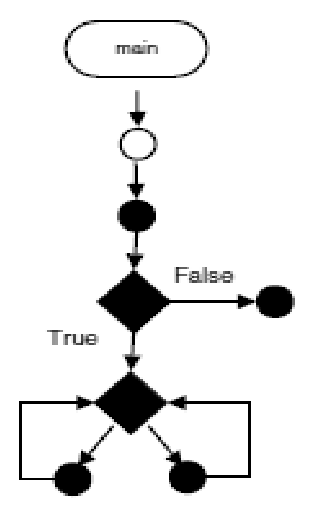
\includegraphics[scale=0.35,clip]{fig/la.eps} 
\caption{\label{fig:la}Example of Look-Ahead (LA) Heuristic} 
\end{figure}

The key idea of the Look-Ahead (LA) heuristic is to perform a reachability analysis in terms of reachable items in the CFG, and decide whether the current
path must be expanded based on the reachability analysis. If no new items can be reached, then exploration along the current path is stopped.

Figure \ref{fig:la} shows an example for illustrating the Look-Ahead (LA) heuristic. Let us assume the depth bound $k \geq 4$ and the objective is to achieve full statement coverage, and every path of the program is feasible. Then the original DFS based produre needs to explore $\approx2^k$ paths to achieve full coverage (because of the two nested loops) while DFS+LA requires at most 3 paths: one path to cover the false branch and two paths to cover two loops.

\subsection{Max-CallDepth (MCD) heuristic}
The major source of path explosion is function calls, and especially nested function calls. It is more embarrassing when only the top-level function is of interest. For example, the procedure may explore alternative (long) paths due to backtrack in deep callees while a simple backtrack at top-level would be sufficient. Example 1 of figure \ref{fig:mcd} gives such a behavior. Figure \ref{fig:mcd2} shows a small program where DFS achieves full branch coverage of main function with $k \geq 8$. DFS+MCD with mcd = 0 and any value of $k$ cannot cover one of the two branches of the main function, since a backtrack in sub-function $f$ is necessary. Consider the program of Figure \ref{fig:mcd}, take mcd = 0 and let us assume that sub-function f does not affect variable b. Then both DFS+LA+UT and DFS+MCD achieve full branch coverage. However, DFS+MCD explores only the two paths of function main, while DFS+LA explores $\approx 2^k$ paths. DFS+LA+MCD performs better
than DFS+LA in the example of Figure \ref{fig:mcd}, and it outperforms DFS+MCD in the example of Figure \ref{fig:la}.

\begin{figure}
\centering
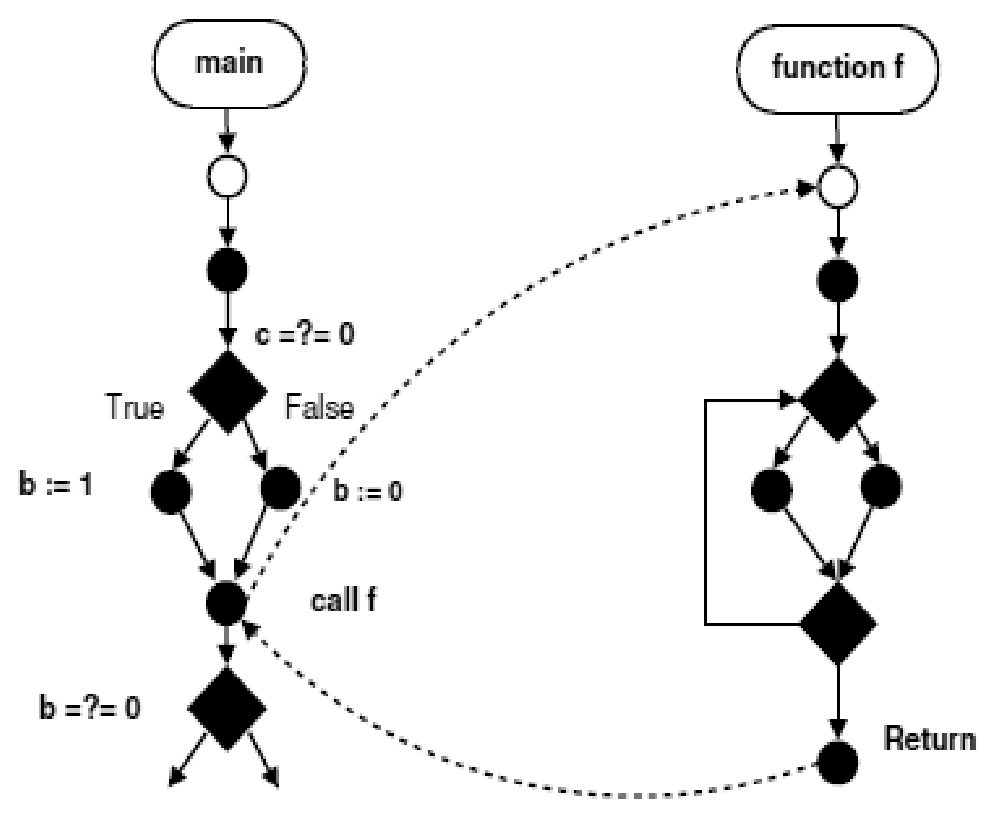
\includegraphics[scale=0.35,clip]{fig/mcd.eps} 
\caption{\label{fig:mcd}Example 1 of Max-CallDepth (MCD) heuristic} 
\end{figure}

The principle of the Max-CallDepth heuristic (MCD) is to prevent backtracking in deep nested calls, hoping such a deep decision is not mandatory to cover the function under test. It is clear that this heuristic makes sense only in unit testing. Moreover, contrary to LA, MCD may discard relevant paths and prevent the full coverage of the function under test. 

\begin{figure}[b]
\centering
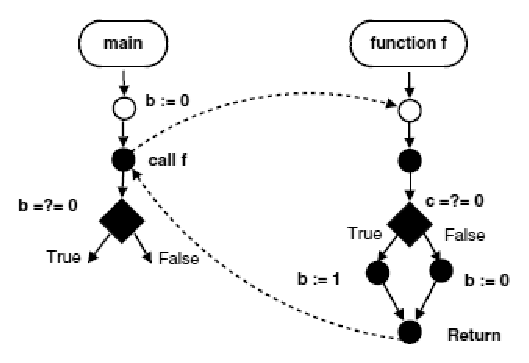
\includegraphics[scale=0.6,clip]{fig/mcd2.eps} 
\caption{\label{fig:mcd2}Example 2 of Max-CallDepth (MCD) heuristic} 
\end{figure}

\subsection{Solve-First (SF) heuristic}
Compared to other graph searches, DFS path exploration lowers memory consumption, since only one path at a time has to be maintained. However, DFS has at least two disadvantages in path-based testing. First, in a realistic environment where the number of tests we can run is limited, DFS may focus only on a very deep and narrow portion of the program under test and achieve only a poor global coverage. Second, DFS-based procedures explore and try to solve first the longest path prefixes, while shorter prefixes with probably simpler constraints may have covered the same items. Hence, DFS suffers from a slow initial coverage-speed and may waste resources on unduly complex paths.

\begin{figure}
\centering
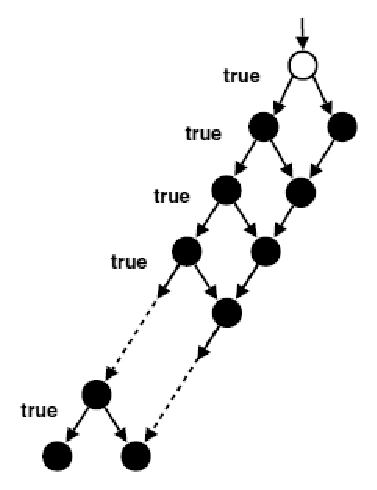
\includegraphics[scale=0.6,clip]{fig/sf.eps} 
\caption{\label{fig:sf}Example of Solve-First (SF) heuristic} 
\end{figure}

Solve-First heuristic (SF) is to partially address both issues described above, while keeping most of the advantages of DFS. SF is a DFS with the slight following modifications. When the procedure reaches a branch (choice point) for the first time, the first successor node is chosen as usual but all alternative successors are immediately resolved. Test data are derived from the solutions and executed in concrete mode to update coverage information. All solutions found are stored in a cache. On backtrack, once the next successor is chosen, the corresponding test
data is retrieved from the cache. The test data is then relaunched and the procedure proceeds as usual in the concolic case.

The program shown in Figure \ref{fig:sf} is parametrized by its number of nodes 2n + 1. Let us assume that all paths are feasible and that the first concrete path goes through every true branch. DFS+LA needs to explore n + 1 paths to achieve full instruction coverage while DFS+LA+SF
needs only to explore 2 paths. The depth bound for the concrete execution may be much larger than the one for concolic execution, allowing to cover more items. Note that essentially SF is concolic and has no interest in a symbolic setting.

\subsection{Conclusion and Related Work}
These three heuristics address the path explosion issue in common cases of irrelevancy. All these heuristics are lightweight, both in terms of implementation cost and computational overhead, and they are all complementary since each one addresses a typical source of path explosion.
Their evaluations show that these heuristics have a significant impact on the number of paths considered and overall performances. Although these three techniques have been presented in a DFS framework, they are easy to adapt to other path-based frameworks. 

Other related works address the problem of path explosion in rather different ways than their heuristic approach. Path explosion due to thread interleaving in concurrent programs is addressed in \cite{distribute, peephole}. The first work is inspired by partial orders methods from (explicit) model checking, while the second work is more ad hoc. Going back to nested function calls, some works have been conducted on modular test generation in order to avoid function inlining. Function summaries are used by recent approaches, which can be either discovered during the static analysis \cite{demand, compositional} or provided manually \cite{allpath}. Functions can also be handled lazily \cite{demand}.



\section{AI in Fault Detection}
A software fault (also called bug) refers to a static defect in the software. When the software is executed with a certain input, a software fault may result in an incorrect internal state, which is referred to as software error. If the software error is propogated to the output of the software, and results in incorrect behaviors with respect to the requirements or other description of the expected behavior, a software failure occurs~\cite{testbook}. 

As the size of complexity of software has grown quickly in past decades, the difficulty of finding and fixng software faults has increased. Among the different types of faults, concurrency faults are the most notorious, due to their non-deterministic nature. Concurrency faults depend not only on inputs and execution environments, but also on threadinterleaving and other timing-related events that are to be manifested, which creates challenges to expose and detect concurrency faults during in-house testing. With the pervasiveness of multi-core machines and concurrent programs, this problem is becoming more and more severe.

Besides concurrency faults, semantic faults are another form of hard-to-detect faults. Typical semantic faults are caused by missing the reassignment of some variables or incorrectly reuse some variables. Such faults are program-specific and difficult to detect by using only in-housing testing. Finally, memory corruption faults such as buffer overflow and dangling pointer are also important, since they can be exploited by malicious users.

To automatically identify such faults, Shi et al.~\cite{wrongDefinition} proposes an approach to first learn the Definition-Use Invariants and then use the learned knowledge of Definition-Use for detecting faults. They observed that regardless of the difference between these faults' root causes, many of them share a common characteristic: when triggered, they usually are followed by an incorrect data flow, i.e., a read instruction uses the value from an unexpected definition, referred to as an incorrect definition. Such commonality indicates that, if we can detect such incorrect definition-use data flow, it is possible to identify these faults automatically, regardless of their different root causes.

Their approach leverages in-house testing as training runs to extract the definition-use invariants. To tolerate insufficient training, their approach automatically prunes out unlikely invariants and violations, and ranks remaining violations based on confidence. Their approach also considers possible training noises (which
may be incorrectly labeled training runs).

\subsection{Definition-Use Invariants}
\textbf{Local/Remote (LR) Invariants.} In concurrent programs, certain read instructions may use only local definitions or only remote definitions (maybe for the purpose of communication or synchronization). LR invariants can be used to describe these properties. Formally speaking, an LR invariant, $LR(r)$, at a read instruction, $r$, equals to “LOCAL” (respectively “REMOTE”) if $r$ uses only definitions from the local (respectively remote) thread. Such invariants are denoted as LR-Local and LR-Remote, respectively. If $r$ can read from either a local or a remote definition, $r$ has no LR invariant. Figure \ref{fig:invariants}(a) illustrates the basic idea of LR invariant.

\begin{figure}
\centering
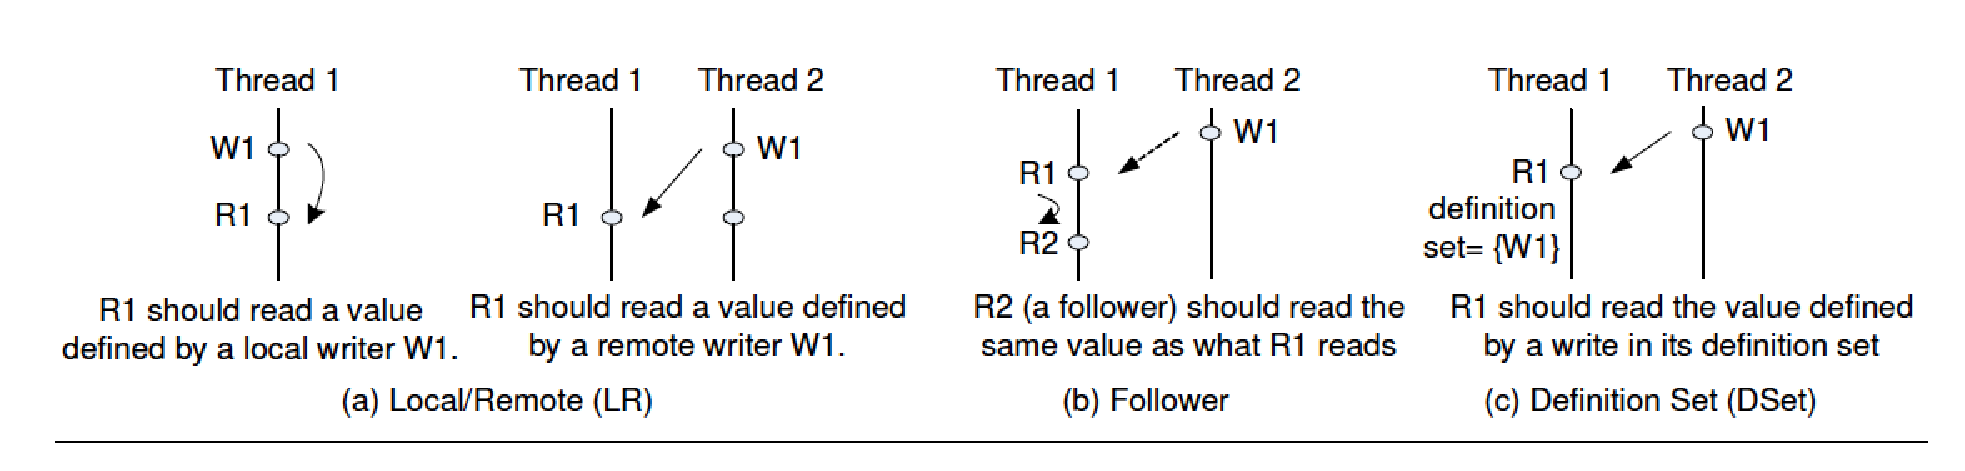
\includegraphics[scale=0.5,clip]{fig/invariants.eps} 
\caption{\label{fig:invariants}Examples of real-world definition-use invariants and their violations.} 
\end{figure}

\textbf{Follower Invariants.} In concurrent programs, developers tend to make assumptions about the atomicity of certain code regions. The LR invariants already captures the case of read-after-write data flow relation in an assumed atomic region, but not the read-after-read case, which can be captured by using a Follower Invariant. Specifically, for two consecutive reads, $r1$ and $r2$, to the same location from the same thread, if $r2$ always uses the same definition as $r1$, $r2$ has a Follower invariant. Follower is different from LR because as long as $r2$ uses the same definition as $r1$, the definition can come from either local or remote. Figure \ref{fig:invariants}(b) demonstrates Follower invariants.

\textbf{Definition Set (DSet) Invariants.} Although concurrent programs have special inter-thread data flows, definition-use is not specific to only concurrent programs. Definition Set (DSet) invariant is suitable for identify faults in both sequential and concurrent programs. A DSet invariant at a read instruction is defined as the set of all write instructions whose definitions this read instruction may use. Figure \ref{fig:invariants}(c) shows a DSet invariant at $R1$. Every read instruction has such a DSet. When an instruction violates a DSet invariant by consuming a value defined by an instruction outside its DSet, this instruction may indicate a likely fault.


\subsection{Invariant Extraction}
To identify faults using definition-use invariants, their approach consists of two phases: (1) an extraction phase for inferring definition-use invariants; and (2) a detection phase for detecting invariant violations and reporting potential faults after pruning and ranking. Figure \ref{fig:overview} shows the overview of their approach.

\begin{figure}[b]
\centering
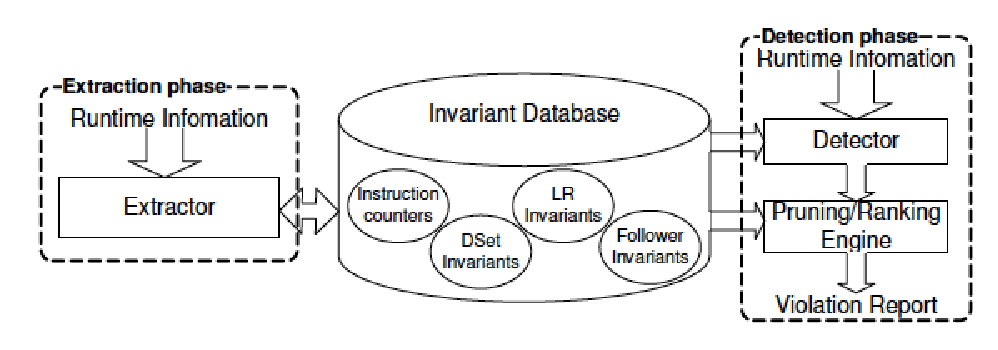
\includegraphics[scale=0.6,clip]{fig/overview.eps} 
\caption{\label{fig:overview}Overview of fault detection using definition-use invariants.} 
\end{figure}

\textbf{DSet invariant extraction}. Their approach obtains DSet by collecting all definitions that are used
by $I_U$ (read instruction) during training runs. For each memory location, their approach stores its most recent $I_D$ (write instruction) in a global hash-table, called Definition-Table. At a read instruction $i_u$, their approach retrieves its definition id from the Definition-Table and uses id's corresponding static instruction ID to update $I_U$'s DSet:

$$ DSet(I_U) \leftarrow DSet(I_U) \bigcup \{I_D\}$$

After the training phase, information for every instructions' DSet is stored into the invariant database along with some statistical information such as the number of times $I_U$ and $I_D$ are executed, and so on. Such statistical information is used for the purpose of pruning and ranking in later phases.

\textbf{LR invariant extraction.} In order to infer LR invariants, their approach first obtains the knowledge of which thread provides the definition for a read instruction by using the Definition-Table. In particular, when $i_u$ is executed, their approach identifies its definition id from the Definition-Table. Their approach then compares the thread identifiers, $T(iu)$ and $T(id)$, to determine whether they are from the same thread or not. Finally, their approach compares the answer with the LR($I_U$) associated with $I_U$. If they are different, LR($I_U$) is set to NO INV to indicate that there is no LR invariant at $I_U$ and this read instruction is no longer monitored for LR invariant extraction. LR($I_U$) is initialized based on the
definition source (either REMOTE or LOCAL) on the first time $I_U$ is executed. This process can be formalized as follows:

\[
LR(I_U) \leftarrow 
\begin{cases}
LOCAL, \text{if } LR(I_U) = LOCAL \wedge T(i_d) = T(i_u)\\
REMOTE, \text{if } LR(I_U) = REMOTE \wedge T(i_d) <> T(i_u)\\
NO\_INV, \text{Otherwise } 
\end{cases}
\]

\textbf{Follower invariant extraction.} To infer Follower invariants, their approach stores its recent access history to determine whether an instruction and its predecessor use the same definition. Their approach maintains a bitvector for every memory location $m$, called has $read(m)$. A bit in the vector has $read(m,t)$ indicates whether the current definition to memory location $m$ has already been used by thread $t$. By checking this bit-vector before every read instruction $i_u$, their approach can easily determine whether $i_u$
and its predecessor use the same definition.

In particular, bit-vector has $read(m)$ is initialized as zero. Every write to $m$ sets all bits of $has\_read(m)$ to zero. After any read from $m$ in thread $t$, $has\_read(m, t)$ is set to one. Before executing a read instruction $i_u$, their approach checks if the corresponding bit (i.e., $has\_read(m,t)$) is one. If it is, it means that there is no new definition since thread $T(i_u)$'s last use to $m$. In other words, $i_u$ shares
the same definition with its predecessor.

To maintain and update the Follower invariant information for $I_U$, their approach associates Follower($I_U$ ) with it. This flag is set to $TRUE$ if $I_U$'s dynamic instances always share definition with their predecessors. Whenever a dynamic instance of $I_U$ uses a different definition from its predecessor, the flag is set to $FALSE$ and $I_U$ is no longer monitored for Follower invariant extraction.

$$ Follower(I_U) \leftarrow Follower(I_U) \wedge has\_read(m,T(i_u))$$


\subsection{Fault Detection}
To detect DSet invariant violation, their approach maintains a Definition-Table at runtime so that it knows which instruction provides a definition for each use. If the definition for a use is not in this use's DSet, a violation is issued. Formally speaking, the violation condition is:
$$I_D \notin DSet(I_U)$$

Detecting violations against LR invariants is also straightforward. At a monitored read, their approach checks whether this read has an LR invariant or not. If it does, their approach examines whether the monitored read and its definition come from the same thread and matches the monitored condition with the type of LR invariant (LOCAL and REMOTE) extracted at this read instruction. 
$$\{LR(I_U) = LOCAL \wedge T(i_d) <> T(i_u)\} \vee \{LR(I_U) = REMOTE \wedge T(i_d) = T(i_u)\}$$

To detect violations to Follower invariants, their appraoch checks whether an instruction with a Follower invariant shares the same definition with its predecessor (by leveraging the has $read(m)$ vector similar to that used in extraction). If not, a violation will be reported.
$$Follower(I_U) \wedge \overline{has\_read(m,T(i_u))}$$

\subsection{Pruning and Ranking}
\textbf{Pruning.} Their approach automatically prunes the following cases: (1) \textit{Barely exercised uses}: For read instructions that are never covered during training, their approach do not report any violations since their approach do not extract any invariants associated with them; (2) \textit{Barely exercised definitions}: For definitions that are never exercised during training runs, their approach also prunes them; (3) \textit{Popular uses}: Some uses, such as those in a small function called from multiple call-sites, are very popular and have a large definition set. In this case, their approach also prunes it as it might be perfectly acceptable to have yet another definition for this use during detection runs.

\textbf{Ranking.} After pruning the above cases, their ranks every unpruned violations based on its confidence. Their approach relies on the following conditions to increase the confidence of a fault: (1) many dynamic instances of the definition ($\#I_D$) and the use ($\#I_U$) during training; (2) no significant difference between the number of instances of the definition and instances of the use ($|\#ID - \#IU|$) during training; (3) small definition set ($|DSet(I_U)|$); (4) few instances of this violation pair ($\#violation_{DSet}(I_D, I_U)$) during detection.

For violations to DSet invariants, their approach computes the confidence using the following formula:
$$conf_{DSet} = \frac{\#I_D \times \#I_U}{(|\#ID - \#IU| \times |DSet(I_U)| \times \#violation_{DSet}(I_D, I_U))}$$

For LR and Follower violations, the confidence is computed based only on the number of dynamic instances of a
use during training and the number of violations occurring during detection, as follows:
$$conf_{LR}=\#I_U / \#violation_{LR}(I_U)$$
$$conf_{F}=\#I_U / \#violation_{F}(I_U)$$

\subsection{Conclusion}
Shi et al.~\cite{wrongDefinition} proposed definition-use invariants which can be used to detect a wide range of software faults, including both concurrency bugs (atomicity and order violations) and sequential bugs (memory corruptions and certain semantic faults). Their experimental results with 16 real-world applications and 20 real-world faults of different types have shown that their approach was effective in detecting 19 of them, including 2 new faults that were never reported before, while introducing only 0-3 false positives. Their training sensitivity experiments showed that their approach can reasonably tolerate insufficient training, especially with confidence-based pruning.

% Recent research works~\cite{wrongDefinition,online} that use AI techniques have advanced the research in reducing the human efforts on fault detection: Shi et al.~\cite{wrongDefinition} proposes an approach to first learn the Definition-Use Invariants and then use the learned knowledge of Definition-Use for detecting concurrency and sequential bugs; Baah et al~\cite{online} and proposes a new machine-learning technique that performs fault detection for deployed software. I plan to study in details how these research works adopt the concepts and techniques of AI to assist the task of fault detection.

\section{AI in Software Repair}
Manual fault fixing is a difficult, time-consuming, labor-intensive process. Some reports place software maintenance, traditionally defined as any modification made on a system after its delivery, at 90\% of the total cost of a typical software project~\cite{modernlegacy}. Modifying existing code, repairing defects,
and otherwise evolving software are major parts of those costs. 

To alleviate the burden, Weimer et al. ~\cite{repair,geneticPatch} introduce a fully automated method
for locating and repairing faults in software. Their approach works on off-the-shelf legacy applications and does not require formal specifications, program annotations or special coding practices. Once a program fault is discovered, an extended form of genetic programming~\cite{genericprogramming} is used to evolve program variants until one is found that both retains required functionality and also avoids the defect in question. Standard test cases are used to exercise the fault and to encode program requirements. After a successful repair has been discovered, it is minimized using structural differencing algorithms and delta debugging.

\subsection{Generic Programming}
Genetic programming (GP) is a computational method inspired by biological evolution, which discovers computer
programs tailored to a particular task~\cite{genericprogramming}. GP operates on and maintains a population comprised of different programs, referred to as individuals or chromosomes. In GP, each chromosome is a tree-based representation of a program. The fitness, or desirability, of each chromosome, is evaluated via an external fitness function. In their paper, fitness is assessed via the test cases. Once fitness is computed, high-fitness individuals are selected to be copied into the next generation. Variations are introduced through
computational analogies to the biological processes of mutation and crossover. These operations create
a new generation and the cycle repeats.

\subsection{Program Representation}
In their approach, each individual (candidate program) is represented as a pair containing:
(1) An abstract syntax tree (AST) including all of the statements in the program; (2) A weighted path through the program under test. The weighted path is a list of pairs, each pair containing a statement in the program and a weight based on that statement�s occurrences in various test cases.

\subsection{Insights}
A biggest impediment for an evolutionary algorithm like GP is the potentially infinite-size search space it must sample to search for a correct program. To address this problem, they introduce two key innovations. First, they restrict the algorithm to only produce changes that are based on structures in other parts of the program. In other words, they hypothesize that a program that is missing important functionality (e.g., a null check) will be able to copy and adapt it from another location in the program. Second, they constrain the
genetic operations of mutation and crossover to operate only on the region of the program that is relevant to the error (that is, the portions of the program that were on the execution path that produced the error). Theses two insights are used together to reduce the search space of software repair.

\subsection{Approach}
To automatically find patches for program repair, their approach uses GP to maintain a population of variants of that program. Each variant is represented as an abstract syntax tree (AST) paired with a weighted program path. Their approach modifies variants using two genetic algorithm operations, \textit{crossover} and \textit{mutation}, specifically targeted to this representation. Each modification produces a new abstract syntax
tree and weighted program path. Their approach then evaluates the fitness of each variant by compiling the abstract syntax tree and running it on the test cases. Its final fitness is a weighted sum of the positive and negative test cases it passes. Their approach stops when a program variant that passes all of the test cases is found. Because GP often introduces irrelevant changes or dead code, their approach further uses tree-structured difference algorithms and delta debugging techniques~\cite{deltadebugging} in a post-processing step to generate a 1-minimal patch that causes it to pass all of the testcases.

\subsection{Conclusion}
Weimer et al.~\cite{geneticPatch,repair} present a fully automated technique for repairing bugs in off-the-shelf legacy software. Rather than using formal specifications or special coding practices, their approach uses an extended form of genetic programming to evolve program variants. Their approach considers only certain classes of repairs, using one part of a program as a template to repair another part. In their GP algorithm, they use a novel representation that combines abstract syntax trees with weighted violating paths; these insights allow their search to scale to large programs. They use standard test cases to show the fault and to encode required functionality; their initial repair is a variant that passes all test cases. The initial repair is minimized using delta debugging and structural differencing algorithm. They are able to generate and minimize repairs for ten different C programs totalling 63,000 lines in under 200 seconds on average.












\bibliographystyle{plain}
\bibliography{references}
\end{document}